
\chapter{Evaluation}
\label{ch:evaluation}

This chapter presents the evaluation of the proposed sampling-based predictive buffer management policy, starting with the evaluation methodology followed by presentation and discussion of results. Note that this is the first implementation and comparison of predictive buffer management policies in an open source system, and PostgreSQL in particular.

\section{Methodology}
Experiments are run on a Ubuntu 20.04.3 LTS server with two 6-core Intel E5-2620v2 CPUs with hyperthreading enabled, 32 GiB of RAM, and a 400 GB Intel S3700 SSD with an ext4 file system. A modified version of BenchBase~\cite{BenchBase} is used as a workload generator for the experiments.
% HDD is: 1 TB ST1000NM0033-9ZM hard drive
% SSD is: 400GB Intel S3700 SSD

% using: `hdparm -i /dev/...`, `sudo lshw -class disk`

Most experiments measure cache hit rate, workload completion time, and I/O volume for different caching policies at different levels of parallelism or with different amounts of memory available. I/O volume isolates the benefits of the improved cache management strategy, while hit rate and run-time provide a more complete picture of the performance. The caching policies compared are PostgreSQL's existing clock-sweep strategy, the PostgreSQL implementation of PBM-PQ, and PBM-sampling configured in a variety of settings.

Hit Rate is measured using PostgreSQL's built-in statistics, automatically retrieved from the \verb|pg_statio_user_tables| system view by BenchBase.

Unless stated otherwise, the available system memory is limited using Linux cgroups. This prevents the OS from caching the entire data set and effectively bypassing secondary storage.

% Each experiment is run multiple times with different random seed for the workload generator. Graphs show the average value with 95\% confidence intervals represented by the error bars.
Each data point plotted is the average from at least 5 independent experiment runs. The error bars show 95\% confidence intervals around the averages.


\section{Sequential Microbenchmarks\label{sec:eval-seq-micro}}





The first set of experiments is a microbenchmark intended to measure the performance impact of the buffer management strategy on sequential- and bitmap-scan heavy workloads. These are similar to the microbenchmarks in \cite{pbm}. %, and serve primarily to compare sampling-based PBM to PBM-PQ on the workloads where PBM-PQ is expected to work well. These are also used to evaluate the impact of additional changes made to the sampling-based strategy.


These experiments are based on TPC-H~\cite{tpch} at scale factor 10. At this scale factor, the \verb|lineitem| table takes approximately 8.6 GiB, and the whole dataset is around 10 GiB without indexes. For this experiment, the \verb|lineitem| table has min-max indexes on the \verb|l_shipdate| column, which is used as the filter for queries, and the table is clustered by \verb|greatest(l_receiptdate, l_commitdate)|. This clustering causes the \verb|l_shipdate| column to be correlated, but not completely sorted, with the physical order, so the min-max index can actually be used effectively. This clustering is to simulate a more realistic physical order than the random order generated by BenchBase's TPC-H implementation. In a real data-set the date columns would correspond with when the row is created or last updated that in turn determines the physical order.\footnote{PostgreSQL generally appends new or updated rows at the end of the table, but can reuse space from previously deleted or updated rows, so the physical order will not perfectly correspond with last-updated time.}

The workload runs several parallel query streams, each executing a fix number of queries. To isolate the impact on a workload with only sequential and bitmap scans, the queries used are modified versions of TPC-H Q1 and Q6 as in \cite{pbm}, which are aggregations on \verb|lineitem| with a filter by \verb|l_shipdate|. Each query uses a different randomly selected range of \verb|l_shipdate| including roughly 30\% of rows in the table.

% For these experiments, the queries are modified versions of TPC-H Q1 and Q6, 
% which only read the \verb|lineitem| table with a filter by \verb|l_shipdate| selecting a random range including roughly 30\% of the rows.

% The \verb|pg_prewarm| postgres extension is used to fill the cache with data from the \verb|lineitem| table before the experiment begins rather than start with an empty cache.



\subsection{Comparing Different Levels of Parallelism}
\label{sec:experiment_micro_parallelism}


% SEQUENTIAL PARALLELISM
\begin{figure}[p]
\centering
\begin{subfigure}{0.45\textwidth}
    \centering
    \includegraphics[width=\textwidth]{figures/seq_micro/Hit rate vs parallelism - Sequential Scan Microbenchmarks.tikz}
    \caption{Effect on Hit Rate}
    \label{fig:seq_micro_parallel_hitrate}
\end{subfigure}\hspace{0.05\textwidth}%
\begin{subfigure}{0.45\textwidth}
    \centering
    \includegraphics[width=\textwidth]{figures/seq_micro/IO volume vs parallelism - Sequential Scan Microbenchmarks.tikz}
    \caption{Effect on I/O Volume}
    \label{fig:seq_micro_parallel_iovol}
\end{subfigure}

\vspace{20pt}
\begin{subfigure}{0.45\textwidth}
    \centering
    \includegraphics[width=\textwidth]{figures/seq_micro/Time vs parallelism - Sequential Scan Microbenchmarks.tikz}
    \caption{Effect on Run-time}
    \label{fig:seq_micro_parallel_time}
\end{subfigure}%\hspace{0.05\textwidth}%
% \begin{subfigure}{0.45\textwidth}
%     \centering
%     % \includegraphics[width=\textwidth]{figures/manual_graphs/seq_runtimes.tikz}
%     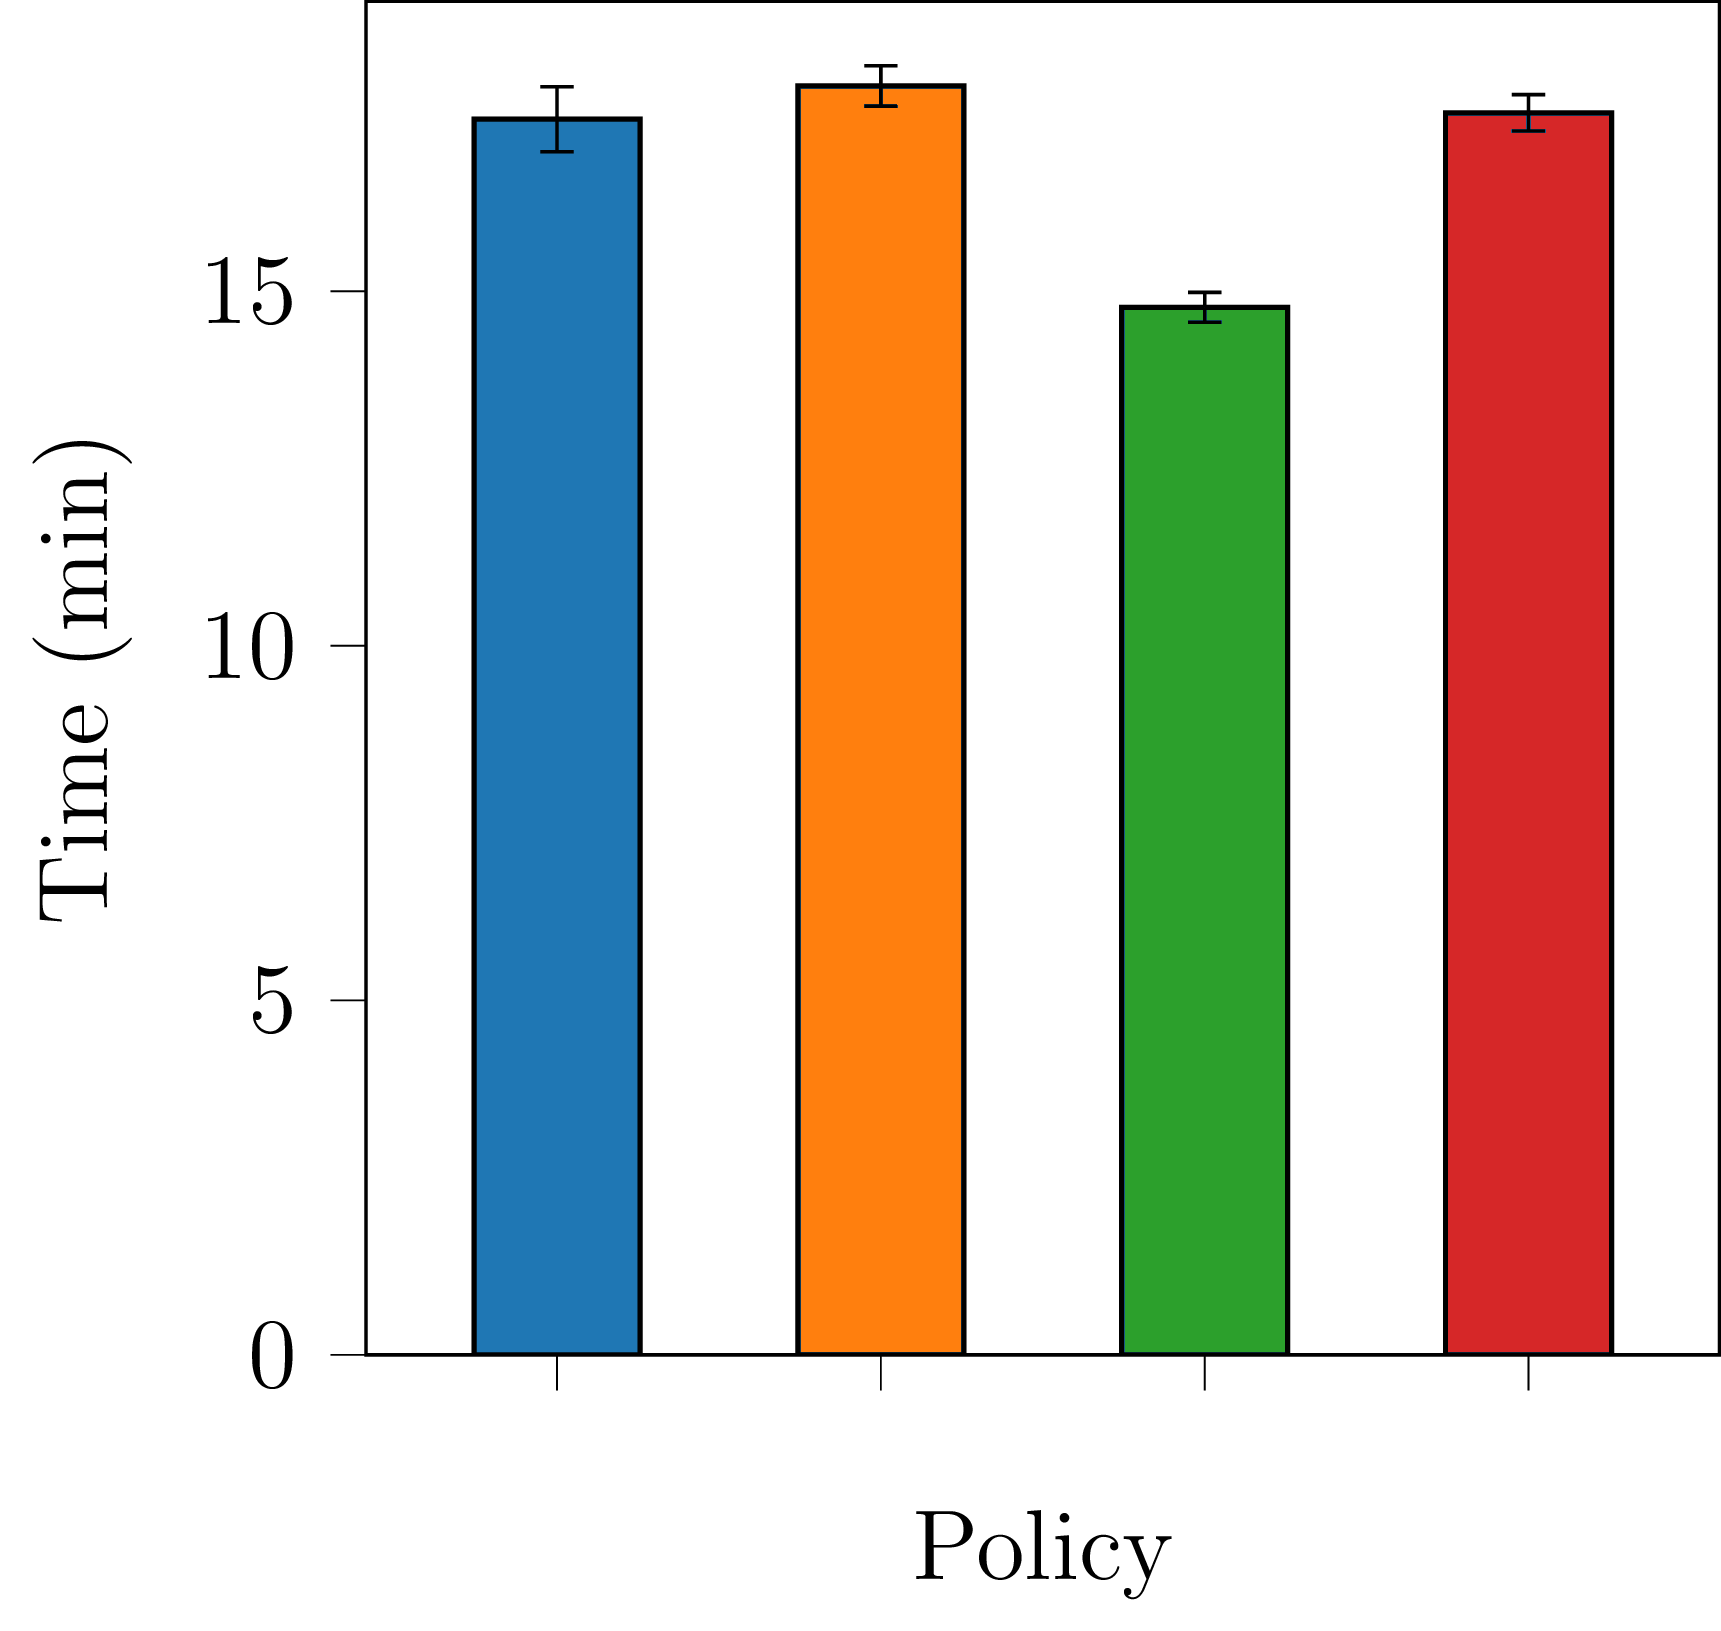
\includegraphics[width=\textwidth]{figures/manual_graphs/seq_runtimes_bar.png}
%     \caption{Run-times at 16 parallelism}
%     \label{fig:seq_micro_runtime_bar}
% \end{subfigure}

\caption{Sequential Microbenchmarks -- Parallelism}
\label{fig:seq_micro_parallelism}
\end{figure}


For this experiment the number of concurrent query streams varies from 1 to 32, with 16 queries per stream each scanning 30\% of the table to measure how the different caching strategies scale with parallelism. PosgtreSQL is configured with 2.5~GiB of cache memory (approximately 30\% of the data size), with available system memory limited to 3~GiB to prevent the OS from caching the whole data set. % some extra memory needed by PostgreSQL for non-cache stuff, hopefully this is obvious enough to not state.

% Revised/additional 2 paras follow.

% Figure~\ref{fig:seq_micro_parallelism} shows the results, with PBM-sampling using 10 samples and no bulk eviction. Since the true test of how well a technique works is how much I/O does its cache management strategy reduce, the focus will be on I/O volume, i.e., I/O savings resulting from using the sampling-based techniques.  To provide a more complete picture, I also show hit rate and workload completion time curves.

% For almost all parallelism levels higher than 2, PBM-sampling delivers significant I/O reductions of about 60 GB over PBM-PQ, which amounts to about 20\% at parallelism level 16 (and 40\% at parallelism level 8 and about 18\% at parallelism level 32).  This I/O reduction is accompanied by higher hit rates and reduced workload completion times. This general trend also holds for the other policies except that PostgreSQL's Clock-Sweep algorithm reduces the gap at parallelism levels higher than 16. 
%  Note that this is the first comparison of all policies against an open source system, and PostgreSQL in particular. 

%  Revised/additional 2 paras ended.
 
Figure~\ref{fig:seq_micro_parallelism} shows the results, with PBM-sampling using 10 samples and no bulk eviction. For all parallelism levels, PBM-sampling without frequency stats delivers significant I/O reductions. At Parallelism level 8 the reduction is about 60 GiB over PBM-PQ, which is nearly 30\% lower, and at parallelism level 32 PBM-sampling saves 11\% I/O volume over PBM-PQ. This I/O reduction is accompanied by higher hit rates and reduced workload completion time. At parallelism levels higher than 16, PostgreSQL's Clock-sweep algorithm pulls ahead of PBM-PQ and reduces the gap but does not entirely catch up with PBM-sampling.

It is interesting to note that at higher parallelism, the hit rates of the different policies seem to be converging along with lower percentage difference in I/O volume and run-time. I believe this is due to scans automatically synchronizing; when two scans are close to each other, the one that is behind will benefit from data loaded into cache by the scan ahead, resulting in a higher hit rate for the scan that is behind allowing it to progress faster and catch up. As the gap closes, the benefit to the trailing scan increases since there is less opportunity for the shared data to be evicted between the two scans. With more parallel queries, the frequency of scans starting close enough together for this situation to occur increases even for simple strategies, reducing the benefits of prediction.

% Comment: "Do you think that the benefit of higher parallelism is proportionally smaller workload completion time, e.g., at around 8 parallelism level, time is 10 mins but at 8x4, it is around 22 and not 4x10 mins?"

% My thoughts: I guess so, maybe better phrased as higher parallelism => higher throughput (but individual query latency also increases)
%  - higher parallelism => better hit-rate, so I/O volume grows sub-linearly
%  - I/O volume is the main factor in run-time for this workload, so run-time doesn't increase linearly either
%  - disk throughput also increases with parallelism, and CPU overhead increases but low parallelism isn't using all the cores so that doesn't grow linearly either

There are some other results supporting this hypothesis: even a purely random eviction strategy tends to get better hit rate at higher parallelism as shown in Figure \ref{fig:seq_micro_parallel_hitrate_samplesize}, and with the data set entirely cached in main memory by the operating system -- so cache misses do not impose a run-time penalty -- the hit rate does not increase in the same way, as show in Figure~\ref{fig:ram_hit_rate}.

\begin{figure}[H]%[h!]
    \centering
    \includegraphics[width=0.5\textwidth]{figures/hdd_ram_micro/Hit rate vs parallelism - RAM Sequential Scan Microbenchmarks.tikz}
    \caption{Sequential Microbenchmarks -- Hit Rate with Data in Main Memory}
    \label{fig:ram_hit_rate}
\end{figure}

Note also that this experiment shows PBM-PQ performing much worse than PBM-sampling, though at low parallelism it out-performs PostgreSQL's clock-sweep strategy. The PostgreSQL implementation of PBM-PQ seems to be more sensitive to changes in the workload and seemingly unrelated parameters, such as block group size, than other policies. %Under some configurations it performs much closer to PBM-sampling.

The data also shows that including the frequency statistics (represented by PBM-sampling + freq in the graphs) as described in Chapter~\ref{sec:frequency-stats} reduces the performance on this workload compared to PBM-sampling without frequency statistics. This is unsurprising, as this workload is one where one would not expect frequency to provide any useful information. The workload already has nearly complete information about relevant future accesses from tracking sequential scans, and blocks accessed multiple times recently are actually \textit{less} likely to be accessed again soon for this workload, since the long-running scans never access the same block more than once. A natural improvement here, which I leave to future work, would be to track how often each table is accessed sequentially versus non-sequentially and ignore frequency statistics for relations that are accessed primarily sequentially. This would remove the penalty of considering frequency statistics when they are not useful (on highly sequential workloads such as this experiment) without sacrificing the benefits of these statistics on less sequential workloads.


\subsection{Comparing Different Cache Sizes}


% SEQUENTIAL CACHE SIZE
\begin{figure}
\centering
    \begin{subfigure}{0.45\textwidth}
    \centering
    \includegraphics[width=\textwidth]{figures/seq_micro/Hit rate vs cache size - Sequential Scan Microbenchmarks.tikz}
    \caption{Effect on Hit Rate}
    \label{fig:seq_micro_shmem_hitrate}
\end{subfigure}\hspace{0.05\textwidth}%
\begin{subfigure}{0.45\textwidth}
    \centering
    \includegraphics[width=\textwidth]{figures/seq_micro/IO volume vs cache size - Sequential Scan Microbenchmarks.tikz}
    \caption{Effect on I/O Volume}
    \label{fig:seq_micro_shmem_iovol}
\end{subfigure}

\vspace{20pt}
\begin{subfigure}{0.45\textwidth}
    \centering
    \includegraphics[width=\textwidth]{figures/seq_micro/Time vs cache size - Sequential Scan Microbenchmarks.tikz}
    \caption{Effect on Run-time}
    \label{fig:seq_micro_shmem_time}
\end{subfigure}

\caption{Sequential Microbenchmarks -- Cache Size}
\label{fig:seq_micro_shmem}
\end{figure}


This experiment runs 8 query streams with 16 queries per stream, and each query scans 30\% of the table. Here the cache size is varied from 0.25 GiB  to 8 GiB, with cgroups limiting the available system memory to the cache size plus 0.5 GiB when cache size is 4 GiB or smaller, and cache size plus 0.6 GiB for larger cache sizes.\footnote{The cache size includes only buffer contents, but each buffer additionally has a metadata header. With a larger cache, PostgreSQL needs a bit of extra space for the extra buffer headers.}

Figure \ref{fig:seq_micro_shmem} shows the results when varying the cache size.
% on hit rate, I/O volume, and run-time.
% Figures \ref{fig:seq_micro_shmem_hitrate} and \ref{fig:seq_micro_shmem_time} show the hit rate and time, respectively, as a function of cache size.
Unsurprisingly, all policies perform better with a larger cache, with the I/O volume and run-time graphs closely matching $(1-\text{hit rate})$ since each different cache size still accesses the same data. PBM-sampling outperforms PBM-PQ and Clock-sweep, with at least an 18\% reduction in I/O volume over each when cache size is at least 2~GiB, and 20\% or more reduction in run-time when cache size is 2 or 3~GiB. As the cache size approaches 100\% of the data size, as expected, the run-time improvements nearly disappear despite the percentage difference in I/O volume increasing between PBM-sampling and PBM-PQ. This is because the I/O volume is very low with a large cache and therefore contributes very little to the run-time. 


\subsection{Impact of PBM-sampling Parameters}
\label{sec:eval_sample_size}


% SEQUENTIAL WITH DIFFERENT SAMPLE SIZES
\begin{figure}
\centering
    \begin{subfigure}{0.45\textwidth}
        \centering
        \includegraphics[width=\textwidth]{figures/seq_micro/Hit rate vs parallelism - Sequential Scans - Impact of Sample Size.tikz}
        \caption{Effect of Sample Size on Hit-Rate}
        \label{fig:seq_micro_parallel_hitrate_samplesize}
    \end{subfigure}\hspace{0.05\textwidth}%
    \begin{subfigure}{0.45\textwidth}
        \centering
        \includegraphics[width=\textwidth]{figures/seq_micro/IO volume vs parallelism - Sequential Scans - Impact of Sample Size.tikz}
        \caption{Effect of Sample Size on I/O Volume}
        \label{fig:seq_micro_parallel_iovol_samplesize}
    \end{subfigure}
    
\vspace{20pt}
    \begin{subfigure}{0.45\textwidth}
        \centering
        \includegraphics[width=\textwidth]{figures/seq_micro/Time vs parallelism - Sequential Scans - Impact of Sample Size.tikz}
        \caption{Effect of Sample Size on Run-time}
        \label{fig:seq_micro_parallel_time_samplesize}
    \end{subfigure}\hspace{0.05\textwidth}%
    \begin{subfigure}{0.45\textwidth}
        \centering
        \includegraphics[width=\textwidth]{figures/manual_graphs/sample_size_runtimes.tikz}
        \caption{\textcolor{blue}{Run-times at 16 parallelism}}
        \label{fig:seq_micro_bar_samplesize}
    \end{subfigure}
    % \begin{subfigure}{0.45\textwidth}
    %     \centering
    %     \includegraphics[width=\textwidth]{figures/seq_micro/Hit rate vs parallelism - Sequential Scans - Impact of Bulk Eviction.tikz}
    %     \caption{Effect of Bulk Eviction on Hit Rate}
    %     \label{fig:seq_micro_parallel_hitrate_bulk}
    % \end{subfigure}
    \caption{Sequential Microbenchmarks -- Parallelism vs Hit Rate with Different PBM-sampling Configurations}
    \label{fig:seq_micro_parallel_samplingparams}
\end{figure}


\begin{figure}

\centering
    \begin{subfigure}{0.45\textwidth}
        \centering
        \includegraphics[width=\textwidth]{figures/seq_micro/Hit rate vs parallelism - Sequential Scans - Impact of Bulk Eviction.tikz}
        \caption{Effect of Bulk Eviction on Hit-Rate}
        \label{fig:seq_micro_parallel_hitrate_bulk}
    \end{subfigure}\hspace{0.05\textwidth}%
    \begin{subfigure}{0.45\textwidth}
        \centering
        \includegraphics[width=\textwidth]{figures/seq_micro/IO volume vs parallelism - Sequential Scans - Impact of Bulk Eviction.tikz}
        \caption{Effect of Bulk Eviction on I/O Volume}
        \label{fig:seq_micro_parallel_iovol_bulk}
    \end{subfigure}
    
\vspace{20pt}
    \begin{subfigure}{0.45\textwidth}
        \centering
        \includegraphics[width=\textwidth]{figures/seq_micro/Time vs parallelism - Sequential Scans - Impact of Bulk Eviction.tikz}
        \caption{Effect of Bulk Eviction on Run-time}
        \label{fig:seq_micro_parallel_time_bulk}
    \end{subfigure}
    \caption{Sequential Microbenchmarks -- Parallelism vs Hit Rate with Bulk Eviction}
    \label{fig:seq_micro_parallel_bulkeviction}
\end{figure}


I repeat the same experiment from Chapter~\ref{sec:experiment_micro_parallelism} but this time compare the impact of sample size and bulk eviction on the performance of PBM-sampling at different levels of parallelism. The ``Random'' policy is PBM-sampling with sample size set to 1.

\Cref{fig:seq_micro_parallel_samplingparams} shows the impact of sample size on the performance of PBM-sampling, varying the number of query streams. For comparing sample size the focus in on hit rate, as this shows the small difference with large sample sizes more clearly than I/O volume. \textcolor{blue}{\Cref{fig:seq_micro_bar_samplesize} shows the run-times as a function of sample size with 16 query streams.}

As expected, more samples results in higher hit rate, and therefore reduced I/O volume and run-time. Interestingly, the diminishing returns of increasing the sample size is demonstrated -- increasing from 20 to 100 samples offers a very small improvement to hit rate (and seemingly no improvement with 32 query streams), less than the improvement from 5 to 10. In contrast to the small improvements at large sample sizes, even just 2 samples provides a significant benefit over random selection.

From the run-time results in Figure~\ref{fig:seq_micro_parallel_time_samplesize}, increased sample size does lead to better over-all performance, and importantly the extra processing overhead of a larger sample size is negligible -- at least at sample sizes under 100.

Figure \ref{fig:seq_micro_parallel_bulkeviction} shows the impact of bulk eviction described in Chapter~\ref{sec:sampling-bulk-eviction} on the performance of PBM-sampling. The graph compares choosing 100 samples and evicting 10 of them to a few different sample sizes with single eviction. Evicting 10 of 100 samples considers the same average number of samples as a sample size of 10 with single-eviction, but the measurements show it performing similarly to a sample size of 20 on this workload. This shows a definite advantage to bulk eviction, achieving better hit rate without increasing the average number of samples -- which is the main factor determining the CPU overhead of sampling.



\section{Trailing Index Scan Microbenchmarks}

% TRAILING INDEX
\begin{figure}
\centering
    \begin{subfigure}{0.45\textwidth}
        \centering
        \includegraphics[width=\textwidth]{figures/idx_trailing/Hit rate vs parallelism - Trailing index scans 1pct.tikz}
        \caption{Hit Rate}
        \label{fig:idx_trailing_hitrate}
    \end{subfigure}\hspace{0.05\textwidth}%
    \begin{subfigure}{0.45\textwidth}
        \centering
        \includegraphics[width=\textwidth]{figures/idx_trailing/IO volume vs parallelism - Trailing index scans 1pct.tikz}
        \caption{I/O Volume}
        \label{fig:idx_trailing_iovol}
    \end{subfigure}
    
\vspace{20pt}
    \begin{subfigure}{0.45\textwidth}
        \centering
        \includegraphics[width=\textwidth]{figures/idx_trailing/Time vs parallelism - Trailing index scans 1pct.tikz}
        \caption{Run-time}
        \label{fig:idx_trailing_runtime}
    \end{subfigure}
    \caption{Trailing Index Scan Results}
    \label{fig:idx_trailing}
\end{figure}


These experiments aim to test the scenario where multiple queries are scanning the same B-tree index concurrently, and thus will access the same blocks in the same order as described in Chapter~\ref{sec:idx_trailing}.

Here each query is an index scan on \verb|lineitem| with a filter on the \verb|l_suppkey| column, which is not correlated with the physical order. Each query scans a randomly selected 1\% range, chosen from a fixed 5\% of the values of the column. Since the column is not correlated with the physical order, this 5\% range covers nearly all the physical blocks and scanning 1\% of the table could access up to half the blocks in the table per query.

Similar to the previous microbenchmarks, the database uses 2.5~GiB of cache with 3~GiB of available system memory. Each query stream executes 6 queries and the number of parallel query streams ranges from 1 to 32.


Figure \ref{fig:idx_trailing} shows the resulting hit rate, I/O volume, and run-time results. Somewhat surprisingly, \gls{pbm} does better than PostgreSQL's existing Clock-sweep approach even without any special support for index scans. PBM-PQ performs slightly better than Clock-sweep, with PBM-sampling doing significantly better than both of them. PBM-sampling reduces I/O volume and run-time by nearly 12\% over PBM-PQ and 15\% over Clock-sweep with 32 query streams. On this workload, PBM-sampling without any extra features (no frequency stats or index support) is simply choosing a random block to evict (and in fact performs the same as an explicitly random policy, though this is not shown in the figure). 

Comparing PBM-sampling with extra features, adding frequency statistics reduces the I/O volume of PBM-sampling by 4-7\% at most levels of parallelism with similar improvements to run-time. Since this experiment touches only 5\% of the rows -- but nearly all the actual blocks -- the frequency statistics identify the blocks that contain more relevant rows than other blocks and prioritize keeping those ones in the cache, explaining the benefits provided.

% Unfortunately, the explicit detection and handling of this situation discussed in Chapter~\ref{sec:idx_trailing} seems to provide no benefit.

% Note: it appears to help at 32 parallelism, but this seems to just be variance in the results. Running at higher parallelism (48, 64) does not show any difference.


\section{Sequential Index Scan Microbenchmarks}


% SEQUENTIAL INDEX
\begin{figure}
\centering
    \begin{subfigure}{0.45\textwidth}
        \centering
        \includegraphics[width=\textwidth]{figures/idx_seq/Hit rate vs parallelism - Sequential index scans.tikz}
        \caption{Hit Rate}
    \end{subfigure}\hspace{0.05\textwidth}%
    \begin{subfigure}{0.45\textwidth}
        \centering
        \includegraphics[width=\textwidth]{figures/idx_seq/IO volume vs parallelism - Sequential index scans.tikz}
        \caption{I/O Volume}
    \end{subfigure}
    
\vspace{20pt}
    \begin{subfigure}{0.45\textwidth}
        \centering
        \includegraphics[width=\textwidth]{figures/idx_seq/Time vs parallelism - Sequential index scans.tikz}
        \caption{Run-time}
    \end{subfigure}

    \caption{Sequential Index Scan Results}
    \label{fig:idx_seq}
\end{figure}

This set of experiments targets the case where the index order is highly correlated with physical order. The setup here is the same as in Chapter~\ref{sec:eval-seq-micro}, except with B-Tree indexes instead of BRIN. The queries, which are also the same as Chapter~\ref{sec:eval-seq-micro}, filter by \verb|l_shipdate|, which is correlated with the physical order of the table. % still use 2.5 GiB of cache, 3 GiB of available system memory, and vary parallelism from 1 to 32, with 8 queries per stream.

Figure \ref{fig:idx_seq} show the results for these experiments. PostgreSQL's existing clock-sweep algorithm performs the best for this workload, followed closely by PBM-sampling with frequency statistics which has 35\% higher I/O volume and 25\% increased run-time at 6 query streams than Clock-sweep, but almost catches up at 32 query streams. Compared to PBM-PQ, however, it reduces I/O volume by 45\% and run-time by 41\% at 32 query streams. Since this workload has no sequential scans, the frequency statistics are the only information used by PBM-sampling to make caching decisions for this configuration. It is not surprising that frequency statistics perform well here. Each blocks will contain data mostly from a small range rather than uniformly distributed over the whole dataset, so block-level accesses will be skewed in a way that is easily picked up by tracking recent accesses.

The \gls{pbm} strategies without any support for index scans predictably do significantly worse, with PBM-PQ performing significantly better than PBM-sampling without frequency statistics. Using sampling without frequency statistics is essentially a purely random policy, since it has no information to inform its decisions on this workload. The PostgreSQL implementation of PBM-PQ behaves similar to FIFO when it has no information about sequential scans, which may explain why it does not do as poorly on this workload as a random policy.


\section{TPC-H}

Some similar experiments based on the TPC-H~\cite{tpch} benchmark are used to test a hybrid workload. These experiments run TPC-H queries 1 through 16\footnote{TPC-H has 22 queries, but the query plans chosen by PostgreSQL for a few of the later queries result in them taking orders of magnitude longer to run than the other queries. Thus those queries are omitted to keep the run-times reasonable and avoid having only one access pattern dominate the workload.} once each in a random order in each query stream. For these experiments, \verb|lineitem| is still clustered based on the date columns and \verb|orders| is clustered base on \verb|o_orderdate|, while the clustering for the other smaller tables is unchanged from the insertion order. A mix of BRIN and B-Tree indexes is used, keeping B-Tree indexes for primary keys and on the \verb|partsupp| table with BRIN on other columns, using min-max indexes for columns used in query predicates that have some correlation with the physical order, and bloom indexes on columns that are used in equality conditions but are not correlated with the physical order. The cache size stays constant at 2.5~GiB with 4~GiB of available system memory as parallelism is changed. The extra system memory compared to the microbenchmarks is required to accommodate extra memory used for joins.

Figure~\ref{fig:tpch_results} shows results comparing different caching policies at different levels of parallelism. With frequency-based estimates included, PBM-sampling is able to match and even slightly exceed the Clock-sweep approach at high parallelism, with 3\% lower I/O volume and 4\% lower run-time at 32 parallelism. PBM-sampling with frequency statistics also achieves 14\% lower I/O volume and run-time compared to PBM-PQ and PBM-sampling without frequency statistics.

Without any extra features, PBM-sampling performs similarly to PBM-PQ, and both perform worse than PostgreSQL's existing clock-sweep algorithm. It is not unexpected that they would under-perform, as this workload involves a lot of index access rather than just sequential access. Considering only sequential and bitmap access causes these strategies to evict blocks accessed mainly through indexes as soon as possible when they should be kept instead.


% TPCH
\begin{figure}
\centering
    \begin{subfigure}{0.45\textwidth}
        \centering
        \includegraphics[width=\textwidth]{figures/tpch/Hit rate vs parallelism - TPCH.tikz}
        \caption{Hit Rate}
        \label{fig:tpch_hitrate}
    \end{subfigure}\hspace{0.05\textwidth}%
    \begin{subfigure}{0.45\textwidth}
        \centering
        \includegraphics[width=\textwidth]{figures/tpch/IO volume vs parallelism - TPCH.tikz}
        \caption{I/O volume}
        \label{fig:tpch_iovol}
    \end{subfigure}
    
\vspace{20pt}
    \begin{subfigure}{0.45\textwidth}
        \centering
        \includegraphics[width=\textwidth]{figures/tpch/Time vs parallelism - TPCH.tikz}
        \caption{Run-time}
        \label{fig:tpch_time}
    \end{subfigure}
    \caption{TPC-H Results}
    \label{fig:tpch_results}
\end{figure}

% When frequency-based estimates are included, however, PBM-sampling is able to match and even slightly exceed the Clock-sweep approach at high parallelism, with 3\% lower I/O volume and 4\% lower run-time at 32 parallelism. PBM-sampling with frequency statistics also achieves 14\% lower I/O volume and run-time compared to PBM-PQ and PBM-sampling without frequency statistics.


% Without frequency statistics or index support, both \gls{pbm} approaches are considering only the sequential and bitmap scans. Thus they end up sabotaging other parts of the workload that use index scans since they wrongfully assume that blocks not requested sequentially will not be used. Including frequency statistics allows PBM-sampling to be somewhat aware of index scans, and brings the performance back on par with Clock-sweep.

